\chapter {BISDN} \label{chap:bisdn} %% chapter 3

\begin{figure} [!htbp]
    \centering
    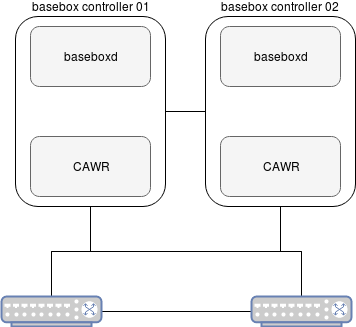
\includegraphics[width=.4\textwidth]{bisdn/basebox}
    \caption{Basebox architecture}
\end{figure}

As the SDN market grows larger and larger in the networking world, new applications and products are developed and improved. Seeing the prevalence of closed source and proprietary solutions for this market, a need for open
products that enable further growth and innovation in cloud DCNs is evident. The main gain in moving from vertically integrated solutions, is the decrease of costs involved, as cheaper solutions can be found in whitebox 
\footnote {whitebox switches are} switches and open sourced networking applications. With this motivation, BISDN developed Basebox, a Linux-powered solution to integrate switches and SDN controllers, allowing for data center 
operators to configure and manage networks using linux commands, removing the need for having to manage several devices with different interfaces and workflows, and adding the capability of running standard networking applications 
on top of the controllers and switches. Basebox also includes the possiblity of running in a failover scenario, by introducing a backup controller for the network, and the possibility of creating a giant switch abstraction, 
by adding another controller, CAWR, and having this manage all the southbound switches.

\par In this chapter we focus on this product, on the first two sections some characteristics of the developed product are described, then we focus on the development of a management API, presenting the required technologies that 
were implemented, and then finally display the results that were obtained in this part of the thesis.

\section {Existing product}

\subsection {baseboxd}
\subsection {CAWR}
